\section{Theorie}
\label{sec:Theorie}
 \subsection{Funktionsweise und Aufbau eines Lock-In-Verstärkers}
  Der Lock-In-Verstärker ist ein Verstärker, der in der Messung stark verrauschter
  Signale eingesetzt wird, indem das Signal von Störfrequenzen bereinigt wird.
  Er hat einen phasenempfindlichen Gleichrichter integriert.
  \begin{figure}
    \centering
    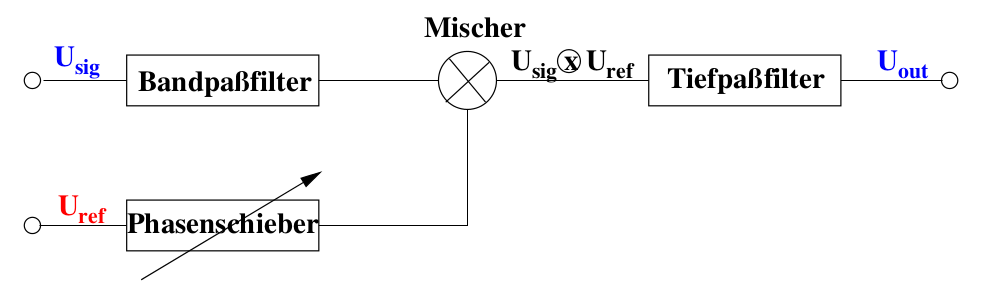
\includegraphics[width=0.8\textwidth]{aufbau.png}
    \caption{Schematischer Aufbau eines Lock-In-Verstärkers\cite{sample}.}
    \label{fig:aufbau}
  \end{figure}
  Der schematische Aufbau eines Lock-In-Verstärkers ist in untenstehender Abbildung
  zu sehen.
  Das verrauschte Nutzsignal $U_\symup{sig}$ wir mit einer Referenzfrequenz $\omega_0$
  moduliert. Dann werden mit einem Bandpassfilter Rauschanteile mit höherer oder
  niedrigerer Frequenz als $\omega_0$ rausgefiltert.
  Es wird nun ein Referenzsignal $U_\symup{ref}$ mit Frequenz $\omega_0$ erzeugt,
  welches im Mischer mit dem Eingangssignal $U_\symup{sig}$ multipliziert wird.
  Damit die beiden Signale synchron sind (also eine Phasenverschiebung
  $\Delta\Phi=0$ haben), kann die Phasenlage $\Phi$ des Referenzsignals mit einem
  Phasenschieber verändert werden.
  Nach dem Mischer wird das resultierende Signal $U_\symup{sig} \times U_\symup{ref}$
  mit einem Tiefpassfilter über mehrere Perioden integriert. Dabei mitteln sich
  die Frequenzbeiträge, die nicht synchron zur Modulationsfrequenz sind, raus.
  Am Ausgang erhält man damit eine Gleichspannung, welche proportional zur
  Eingangspannung $U_\symup{sig}$ ist. Es gilt
  \begin{equation}
    U_\symup{out}\propto U_0\, cos\,\Phi.
    \label{eqn:porportionalitaet}
  \end{equation}
  $U_\symup{out}$ wird also maximal, wenn für die Phasenverschiebung
  $\Delta\Phi=k\cdot2\pi$ mit $k\in\symbb{Z}$ gilt, da der Kosinus dann maximal ist.
  Ein Lock-In-Verstärker kann eine Güte von $Q=100000$ erreichen, da die Bandbreite
  $\Delta\nu = \frac{1}{\pi RC}$ des Tiefpasses sehr klein wird, wenn eine große
  Zeitkonstante $\tau=RC$ gewählt wird.
  Die Güte des Lock-In-Verstärkers ist um einen Faktor von 100 größer, als wenn
  das Signal nur mit einem Bandpass gefiltert würde.
  \newpage
  \subsection{Signalverläufe}
  Als Eingangssignal liegt eine sinusförmige Signalspannung
  \begin{equation}
    U_\symup{sig} = U_0 \sin(\omega t)
    \label{eqn:usig}
  \end{equation}
  vor, welche mit einer Rechteckspannung $U_\symup{ref}$, die eine Amplitude von
  1 hat, multipliziert wird.
  Die Rechteckspannung wird mit einer Fourierreihe genähert, welche nur die ungeraden
  Harmonischen der Grundfrequenz $\omega$ enthält:
  \begin{equation}
    U_\symup{ref}=\frac{4}{\pi}\left(\sin(\omega t) + \frac{1}{3}\sin(3\omega t)
    + \frac{1}{5}\sin(5\omega t) + \ldots\right).
    \label{eqn:uref}
  \end{equation}
  Für das gemischte Signal ergibt sich mit \eqref{eqn:usig} und \eqref{eqn:uref}
  \begin{equation}
    U_\symup{sig}\times U_\symup{ref} = \frac{2}{\pi}\left(1-\frac{2}{3}\cos(2\omega t)
    -\frac{2}{15}\cos(4\omega t) -\frac{2}{35}\cos(6\omega t) - \ldots\right),
    \label{eqn:umisch}
  \end{equation}
  \begin{wrapfigure}{r}{0.45\textwidth}
    \centering
    \vspace{-15pt}
    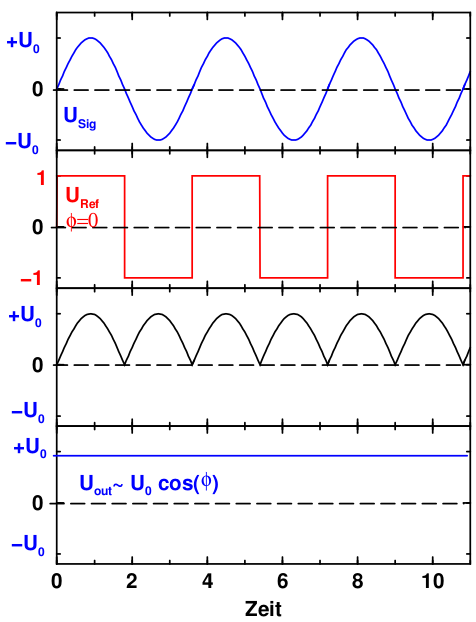
\includegraphics[width=0.4\textwidth]{signalverlaeufe.png}
    \caption{Signalverläufe\cite{sample}.}
    \label{fig:signalverlaeufe}
  \end{wrapfigure}
  welches nur gerade Oberwellen der Grundfrequenz $\omega$ enthält.
  Der Tiefpass eleminiert nun die verbliebenen Oberwellen, so dass man als Ausgangssignal
  eine zur Eingangssignalspannung proportionale Gleichspannung
  \begin{equation}
    U_\symup{out}=\frac{2}{\pi}\,U_0 \cos\,(\Phi)
    \label{eqn:uout1}
  \end{equation}
  erhält. Dabei ist $\Phi$ die Phasendifferenz zwischen Signal- und Referenzspannung.
  Für $\Phi = 0$ vereinfacht sich die Gleichung wegen $\cos(0)=1$ zu
  \begin{equation}
    U_\symup{out}=\frac{2}{\pi}\,U_0.
    \label{eqn:uout2}
  \end{equation}
  Für diesen Fall ist die Ausgangsspannung maximal.
\cite{sample}
